\documentclass[conference, a4paper]{IEEEtran}
\IEEEoverridecommandlockouts

\usepackage{cite}
\usepackage{amsmath,amssymb,amsfonts}
\usepackage{algorithmic}
\usepackage{graphicx}
\usepackage{textcomp}
\usepackage{xcolor}
\usepackage{float}
\usepackage{caption}
\usepackage{subcaption}

\graphicspath{{../../graphics}{../../graphics/planar_dielectric_waveguide}{../../graphics/rectangular_dielectric_waveguide}{../../graphics/comsol_individual_waveguide}}

\def\BibTeX{{\rm B\kern-.05em{\sc i\kern-.025em b}\kern-.08em
    T\kern-.1667em\lower.7ex\hbox{E}\kern-.125emX}}
\begin{document}

\title{Coupled Mode Theory and 50/50 Splitter}

\author{\IEEEauthorblockN{Eduardo A. V. Souza, RA: 250950}
\IEEEauthorblockA{\textit{"Gleb Wataghin" Institute of Physics} \\
\textit{UNICAMP}\\
Campinas, Brazil}
\and
\IEEEauthorblockN{Ivan Prearo (RA 237215)}
\IEEEauthorblockA{\textit{"Gleb Wataghin" Institute of Physics} \\
\textit{UNICAMP}\\
Campinas, Brazil}}

\maketitle

\begin{abstract}
    In this work, we aimed to design a 50/50 splitter made a two-waveguide coupled system. First, we started with a pre-analysis with COMSOL to optimize the material of the waveguides, their width and thickness, alongside with a resonable gap to obtain a short in length splitter. Then, we followed to the theoretical modeling of the problem based on Coupled Mode Theory, ranging from the derivation of the coupling constant formula, the coupled mode equations, and a numerical method to calculate the coupling rate. At the end, we analysed two cases of beamplitter, the first with identical waveguides, and the second with one waveguide with doubled dimensions. We found that the second case is better to obtain a more compact splitter.
\end{abstract}

\begin{IEEEkeywords}
    Waveguides, Coupled Mode Theory, Beamsplittersnsing.
\end{IEEEkeywords}

\section{Introduction}
\label{sec:intro}

In this section, we aim to describe the investigation to choose the material and the geometrical parameters of the waveguides belonging the coupled system. In the first place, we considered $SiO_2$, $TiO_2$, $Si_3N_4$, and $Ag_3AsS_3$ as the possible materials due to their renowed applications in photonic integrated circuits (PIC). Fig. \ref{fig:dispersion} displays the dispersion of each one of these materials. As it is evident, $Ag_3AsS_3$ has the greatest values of refracive index (RI) and $SiO_2$ has the lowest, while $TiO_2$ and $Si_3N_4$ are intermediate cases. 

\begin{figure}[H]
    \centering
    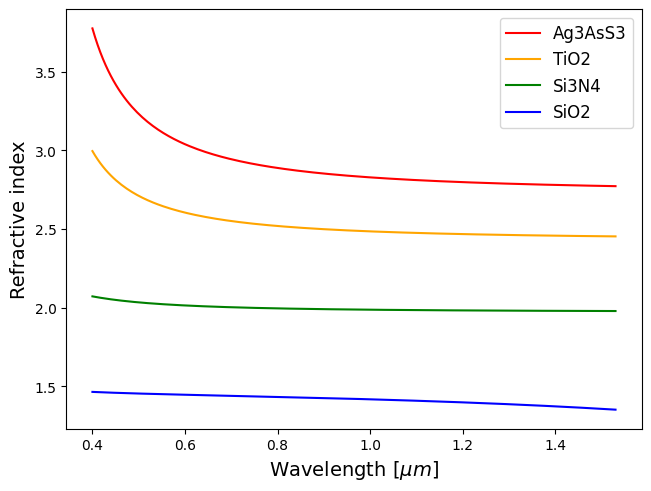
\includegraphics[scale=0.4]{dispersion_relation.png}
    \caption{Dispersion relation for the $SiO_2$, $TiO_2$, $Si_3N_4$, and $Ag_3AsS_3$.}
    \label{fig:dispersion}
\end{figure}

Motivated by the common use of $SiO_2$ and $TiO_2$ in waveguides, and the info they present distinctive dispersion relations, $TiO_2$ presenting the highest values, we will focus on these materials as the candidates for the beam splitter. So, their dispersion relations are described by Eq. \eqref{eq:dispersion}.

\begin{subequations}
    \begin{align}
        n_{SiO_2} &= 
        \sqrt{\begin{aligned}[t]
            &1 + \frac{0.6961663 \lambda^2}{\lambda^2 - 0.0684043^2} 
            + \frac{0.4079426 \lambda^2}{\lambda^2 - 0.1162414^2} \\
            &+ \frac{0.8974794 \lambda^2}{\lambda^2 - 9.896161}
        \end{aligned}}
    \end{align}
    \begin{align}
        n_{TiO_2} &= \sqrt{5.913 + \frac{0.2441}{\lambda^2 - 0.0803}}
    \end{align}
    \label{eq:dispersion}
\end{subequations}

To understand the number of modes in a waveguide with these materials, we plotted the characteristic equations for each material for the infinite dielectric slab case, which has a easier mathematical description. The generic characteristic equation is described by Eq. \eqref{eq:char_equation}, and the case for $SiO_2$ is plotted in Fig. \ref{fig:char_equation}.

\begin{equation}
    \begin{split}
        f_1(\sin(\theta)) 
        &\equiv \tan\left[ \pi \left(\frac{\sin(\theta) d}{\lambda} - \frac{m}{2}\right) \right] \\
        &= \sqrt{\frac{\sin^2(\overline{\theta}_c)}{\sin^2(\theta)} - 1} \equiv f_2(\sin(\theta))
    \end{split}
    \label{eq:char_equation}
\end{equation}


\begin{figure}[H]
    \centering
    \centering
    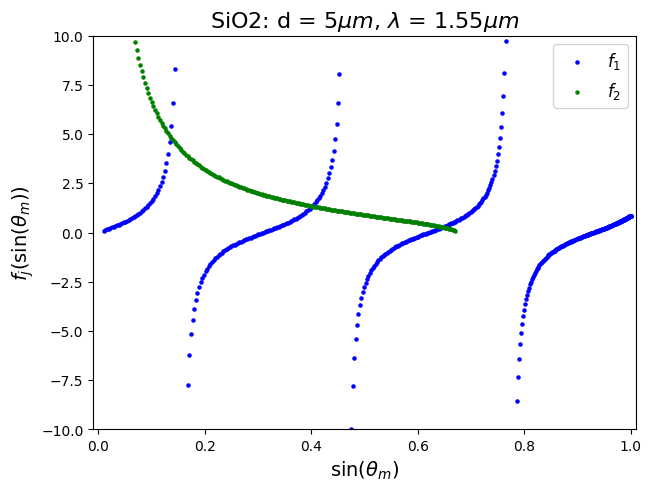
\includegraphics[scale=0.4]{modes_SiO2_d5um_wv1.55um.png}
    \caption{$SiO_2$.}
    \caption{Plot of the characteristic equations for the $SiO_2$ and $TiO_2$ infinite slab case.}
    \label{fig:char_equation}
\end{figure}




\section{Infinite dielectric waveguide}
\label{sec:slab}

\subsection{Theory development}
\label{subsec:slab_theory}

\subsection{Numerical analysis}
\label{subsec:slab_num}

\section{Rectangular dielectric waveguide}
\label{subsec:rectangle}

\subsection{Theoretical development}
\label{subsec:rectangle_theory}

\subsection{Solo waveguide}
\label{subsec:rectangle_solo}

\begin{figure}[H]
    \centering
    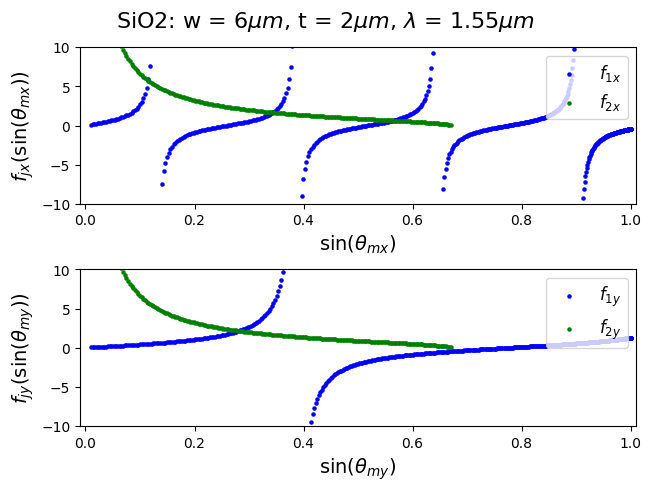
\includegraphics[scale=0.5]{characteristic_equation_SiO2.png}
    \caption{}
    \label{fig:cha_eq}
\end{figure}

\begin{figure}[H]
    \centering
    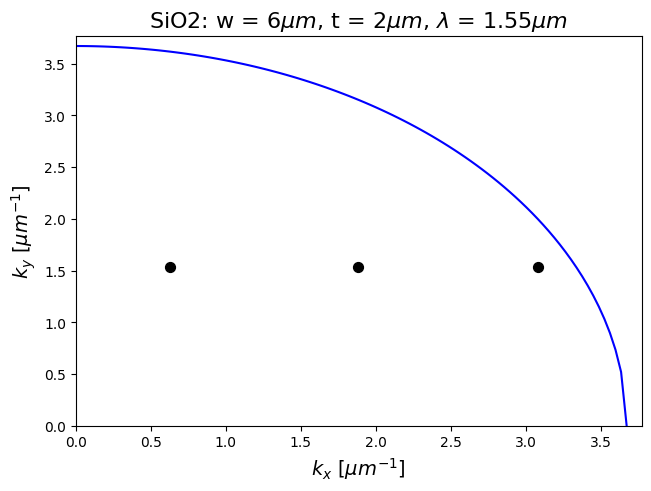
\includegraphics[scale=0.5]{modeshell_SiO2.png}
    \caption{}
    \label{fig:mode_shell}
\end{figure}

\begin{figure}[H]
    \centering
    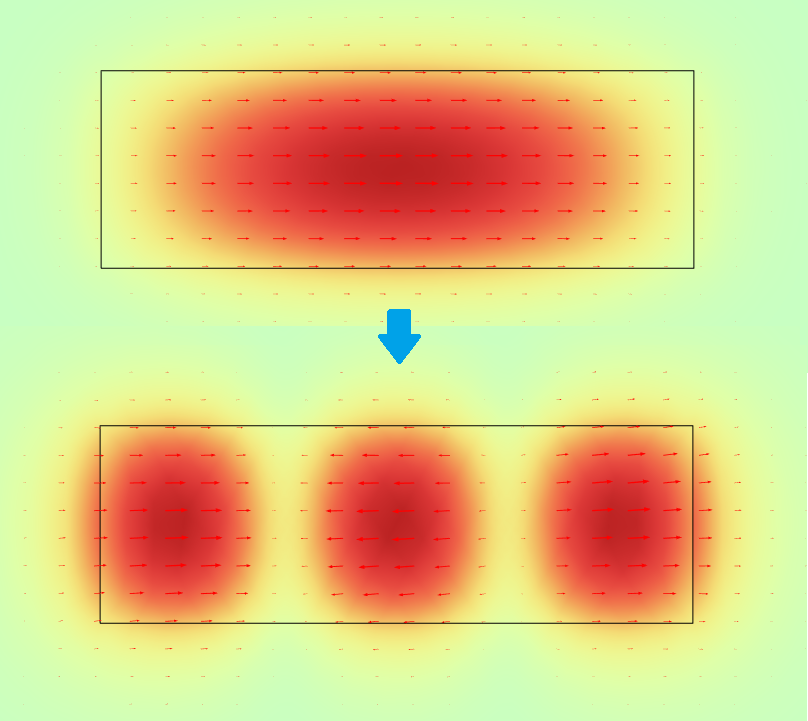
\includegraphics[scale=0.3]{normE_different_modes.png}
    \caption{}
    \label{fig:dif_modes}
\end{figure}

\subsection{Coupled waveguide}
\label{subsec:rectangle_coupled}

\section{Conclusion}
\label{sec:conclusion}

\section*{Appendix}
\label{sec:appendix}

% \bibliographystyle{IEEEtran}
% \bibliography{References}


\end{document}
